% Telemetría, dashboard, API y Modbus: común a los manuales (se incluye con \input)
\section{Telemetría, dashboard, API y Modbus}\label{sec:datos}
Además de mostrar y mandar el brazo, la app guarda lo que pasa y lo publica para otros programas. Nada de esto es obligatorio: si falta la base de datos, la app funciona igual y solo guarda los archivos CSV.

\subsection{Qué se guarda}
\begin{itemize}
\item \textbf{CSV, siempre}: un archivo por sesión en la carpeta \codigo{telemetria/}, con nombre \codigo{telemetria\_\-AAAAMMDD\_\-HHMMSS.csv} y una fila por segundo: posición de la base y de los carros, frecuencia de los trenes de pulsos, entradas y salidas.
\item \textbf{PostgreSQL, si está instalado} (la instalación de la base está en los manuales de Linux y de Windows): una muestra por segundo y por variable (tags ZI-101 a ZI-103, SY-100 y SY-101), los cambios de cada señal del PLC, las alarmas (errores del PLC y pérdida de comunicación), las órdenes con quién las dio y si se aceptaron, y los ingresos de los usuarios. Cada modo elegido en el menú abre un \emph{ciclo de operación}.
\end{itemize}
La lectura del PLC y el guardado corren por separado: una base lenta o caída no frena el gemelo ni la vigilancia del PLC. Para no guardar nada, abra la app con \codigo{-{}-sin-telemetria}.

\subsection{Dashboard}
El botón \emph{Dashboard} de la barra superior abre el tablero de la planta (también en \codigo{/dashboard.html} desde la red):
\begin{figure}[H]
\centering
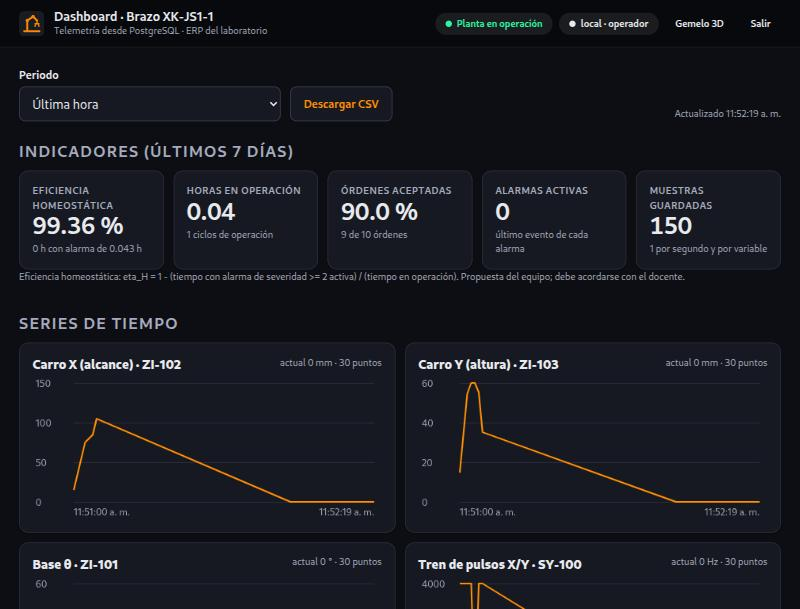
\includegraphics[width=0.85\linewidth]{img/dashboard.jpg}
\caption{Dashboard: indicadores de los últimos 7 días y series de tiempo de cada eje.}
\end{figure}
\begin{itemize}
\item \textbf{Indicadores}: eficiencia homeostática (fracción del tiempo de operación sin alarmas graves), horas de operación, órdenes aceptadas, alarmas activas y muestras guardadas.
\item \textbf{Series de tiempo} de la base, de los carros y de los trenes de pulsos, para la última hora, el último día o la última semana, con un botón para descargarlas en CSV.
\item \textbf{Tablas} de alarmas, órdenes e ingresos.
\end{itemize}
Un usuario observador ve el dashboard pero no las sesiones de los demás. El dashboard necesita PostgreSQL: sin base muestra que no hay datos.

\subsection{API para otros programas}
Otros programas (el ERP del laboratorio, una planilla, un script) leen los datos con la API, por la misma dirección del acceso por red:
\begin{lstlisting}
POST /api/v1/token            {"usuario": "ana", "clave": "..."}   ->  {"token": "..."}
GET  /api/v1/telemetria/planta/1?tag=ZI-102&desde=2026-11-24T08:00&formato=csv
GET  /api/v1/alertas/activas     /api/v1/kpi?dias=7     /api/v1/ciclos
GET  /api/v1/ordenes             /api/v1/sesiones (solo operador)
\end{lstlisting}
Cada consulta lleva el encabezado \codigo{Authorization: Bearer <token>}. Sin token, o con una clave errónea, la respuesta es 401; un observador que pide algo reservado al operador recibe 403. La API solo lee: mover el brazo sigue siendo cosa de la ventana del gemelo.

\subsection{Modbus TCP}
Con la opción \codigo{-{}-modbus} la app publica el estado del brazo como esclavo Modbus TCP en el puerto 5020, \textbf{solo lectura}, para un HMI o SCADA:
\begin{center}\small
\begin{tabular}{@{}lll@{}}
\toprule
\textbf{Registro} & \textbf{Tag} & \textbf{Contenido}\\
\midrule
40001--40002 & ZI-101 & posición de la base [pulsos, entero de 32 bits]\\
40003--40004 & ZI-102 & posición del carro X [pulsos]\\
40005--40006 & ZI-103 & posición del carro Y [pulsos]\\
40007 / 40008 & SY-100 / SY-101 & frecuencia del tren X/Y y de la base [Hz]\\
40009 / 40010 & -- & entradas I0.0--I1.5 y salidas Q0.0--Q0.7 (un bit cada una)\\
40011--40013 & ZI-101..103 & base [0,1°], carro X y carro Y [0,1 mm]\\
40014 & -- & estado: conectado, referenciado, en movimiento, garra cerrada\\
40015 & -- & contador de lecturas (cambia mientras la pasarela está viva)\\
\bottomrule
\end{tabular}
\end{center}
Para comprobarlo desde otra PC (muestra los valores y la tasa de error):
\begin{lstlisting}
python3 modbus.py cliente --tcp IP:5020 --repetir 100
\end{lstlisting}

